\section*{Assignment 02: Network Effects and Launch Strategy}
\addcontentsline{toc}{section}{Assignment 02: Network Effects and Launch Strategy}

\subsection*{How we engineered the loops}
SkillSync only works if students and organisations keep nudging each other, so we mapped the network effects explicitly rather than hoping they appear by magic. The cross-side loop is obvious: vetted NGO projects attract impact-hungry students, and their turnout convinces resource-strapped organisations to post again. On top sit two supportive loops: a student same-side effect driven by peer stories, leaderboard shout-outs, and cohort feedback rituals \citep{Choudary2016}; and a data loop where each completed match enriches our skill taxonomy and matching algorithm, nudging us toward the curated-orchestrator archetype from \citet{Reillier2017}.

\subsection*{Breaking the penguin problem}
The penguin problem hit us hard: no student wants to join before credible projects show up, yet NGOs hesitate without proven talent. We attacked it in three coordinated moves. Step one was to partner with two anchor NGOs who already mentored students informally; their endorsements provided the social proof \citet{HagiuWright2013} say you need to seed a young platform. Step two was to recruit a ``founding cohort'' of 40 students via faculty recommendations and give them concierge onboarding, stipends for the first deliverables, and a Slack space moderated by us. Step three layered lightweight guarantees: projects launched with pre-filled briefs, and we promised replacement support if a match fizzled. These subsidies mirror the playbooks from \citet{Gunasilan2024} and \citet{FarrellSaloner1986} on reducing switching risk when nobody wants to move first, and they follow the Session~4 guidance on solving the chicken-and-egg problem \citep{Lecture04}.

\subsection*{Launch strategy reflections}
Looking back, our soft launch favoured breadth over intensity. We opened the waitlist broadly and then scrambled to curate projects, which diluted the feeling of a vibrant community. If we reran it, I would narrow the first wave to one faculty and a handful of NGOs, mirroring the focused-cluster approach advocated by \citet{Choudary2016}. I would also front-load measurement on time-to-first-value and project completion rate so we react faster when loops drag \citep{ShapiroVarian1999}. Finally, we would invest earlier in student ambassadors embedded in each programme; when network effects rely on trust, credible peer voices beat email blasts every time.

Figure~\ref{fig:application-flow} shows the application flow that holds the loops together. The polished `Student-Submission.png` walkthrough lets students browse curated projects, submit a tailored pitch, and immediately see application status. We stripped anything resembling a ``post and pray'' UX to avoid low-effort spam, and the step indicators plus guidance chips reuse mentoring language so the tone stays human.

\begin{figure}[h]
  \centering
  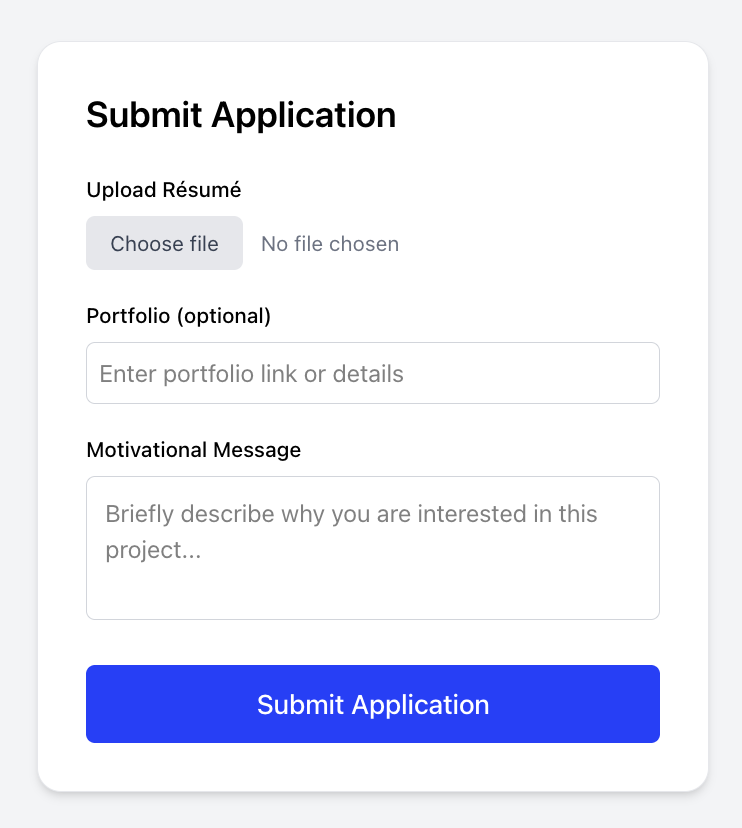
\includegraphics[width=0.75\linewidth]{figures/Student-Submission.png}
  \caption{End-to-end student application flow (`Student-Submission.png`) used to trigger the first successful loops.}
  \label{fig:application-flow}
\end{figure}

I also revisited the organisational journey after the first dozen projects wrapped up. Figure~\ref{fig:project-creation} (in Assignment~3) shows the scoping prompts that keep briefs from arriving half-baked. Behind the scenes Zapier automations alert the founding cohort when new projects drop, pushing acceptance time under 24 hours. We should have built that earlier---Assignment~08's metrics show delay kills repeat usage---so the lesson is clear: seeding relies on choreography and tooling as much as subsidies.
